\documentclass[10pt, a5paper]{article}
\usepackage{pdfpages}
\usepackage{parallel}
\usepackage[T2A]{fontenc}
\usepackage{ucs}
\usepackage[utf8x]{inputenc}
\usepackage[polish,english,russian]{babel}
\usepackage{hyperref}
\usepackage{rotating}
\usepackage[inner=2cm,top=1.8cm,outer=2cm,bottom=2.3cm,nohead]{geometry}
\usepackage{listings}
\usepackage{graphicx}
\usepackage{wrapfig}
\usepackage{longtable}
\usepackage{indentfirst}
\usepackage{array}
\newcolumntype{P}[1]{>{\raggedright\arraybackslash}p{#1}}
\frenchspacing
\usepackage{fixltx2e} %text sub- and superscripts
\usepackage{icomma} % коскі ў матэматычным рэжыме
\PreloadUnicodePage{4}

\newcommand{\longpage}{\enlargethispage{\baselineskip}}
\newcommand{\shortpage}{\enlargethispage{-\baselineskip}}

\def\switchlang#1{\expandafter\csname switchlang#1\endcsname}
\def\switchlangbe{
\let\saverefname=\refname%
\def\refname{Літаратура}%
\def\figurename{Іл.}%
}
\def\switchlangen{
\let\saverefname=\refname%
\def\refname{References}%
\def\figurename{Fig.}%
}
\def\switchlangru{
\let\saverefname=\refname%
\let\savefigurename=\figurename%
\def\refname{Литература}%
\def\figurename{Рис.}%
}

\hyphenation{admi-ni-stra-tive}
\hyphenation{ex-pe-ri-ence}
\hyphenation{fle-xi-bi-li-ty}
\hyphenation{Py-thon}
\hyphenation{ma-the-ma-ti-cal}
\hyphenation{re-ported}
\hyphenation{imp-le-menta-tions}
\hyphenation{pro-vides}
\hyphenation{en-gi-neering}
\hyphenation{com-pa-ti-bi-li-ty}
\hyphenation{im-pos-sible}
\hyphenation{desk-top}
\hyphenation{elec-tro-nic}
\hyphenation{com-pa-ny}
\hyphenation{de-ve-lop-ment}
\hyphenation{de-ve-loping}
\hyphenation{de-ve-lop}
\hyphenation{da-ta-ba-se}
\hyphenation{plat-forms}
\hyphenation{or-ga-ni-za-tion}
\hyphenation{pro-gramming}
\hyphenation{in-stru-ments}
\hyphenation{Li-nux}
\hyphenation{sour-ce}
\hyphenation{en-vi-ron-ment}
\hyphenation{Te-le-pathy}
\hyphenation{Li-nux-ov-ka}
\hyphenation{Open-BSD}
\hyphenation{Free-BSD}
\hyphenation{men-ti-on-ed}
\hyphenation{app-li-ca-tion}

\def\progref!#1!{\texttt{#1}}
\renewcommand{\arraystretch}{2} %Іначай формулы ў матрыцы зліпаюцца з лініямі
\usepackage{array}

\def\interview #1 (#2), #3, #4, #5\par{

\section[#1, #3, #4]{#1 -- #3, #4}
\def\qname{LVEE}
\def\aname{#1}
\def\q ##1\par{{\noindent \bf \qname: ##1 }\par}
\def\a{{\noindent \bf \aname: } \def\qname{L}\def\aname{#2}}
}

\def\interview* #1 (#2), #3, #4, #5\par{

\section*{#1\\{\small\rm #3, #4. #5}}

\def\qname{LVEE}
\def\aname{#1}
\def\q ##1\par{{\noindent \bf \qname: ##1 }\par}
\def\a{{\noindent \bf \aname: } \def\qname{L}\def\aname{#2}}
}

\begin{document}
\title{Testing your distribution automatically in LAVA\footnote{\url{andrew@shadura.me}, \url{https://lvee.org/en/abstracts/264}}}
\author{ Andrej Shadura, Bratislava, Slovakia}
\maketitle
\begin{abstract}
LAVA is a continuous integration system for deploying operating systems onto physical and virtual hardware for running tests. With LAVA, it is possible to run automated tests across multiple hardware platforms in the real operating system environment. LAVA powers the infrastructure behind Kernel CI project,\linebreak ensuring the Linux kernel is tested on as much hardware as possible without human intervention.

This talk will cover LAVA in general and its benefits in the CI process and how it can fit with on your CI infrastructure, and how we at Collabora use it to test Linux distribution images.
\end{abstract}
\section*{Testing distributions with LAVA}

LAVA is a continuous integration system for deploying operating systems onto physical and virtual hardware for running tests. With LAVA, it is possible to run automated tests across multiple hardware platforms in the real operating system environment. LAVA powers the infrastructure behind Kernel CI project, ensuring the Linux kernel is tested on as much hardware as possible without human intervention.

This talk will cover LAVA in general and its benefits in the CI process and how it can fit with on your CI infrastructure, and how we at Collabora use it to test Linux distribution images.

\subsection*{What is LAVA?}

LAVA stands for Linaro Automated Validation Architecture. It\linebreak allows deploying a real-world environment (e.g. OS and other required parts of the system) and the application to a device your software is supposed to run on, and running tests there.

LAVA works by powering on the target device (e.g. a development board, server, virtual machine or any other type of a device), booting an operating system on it, running some commands on it (e.g. tests), recording the output of the commands, powering it off and sending the results back so that they can be analysed. Devices under test are connected using a serial console, they typically have Ethernet network connectivity, and remotely controllable power supplies, so that LAVA can automatically turn them on and off as needed.

The whole process is described by a YAML file defining a pipeline of multiple steps, each of them can be one of \verb@deploy@, \verb@boot@ or \verb@test@. The definition of each step tells LAVA e.g. where to get images, where to put them, how to boot the device and what tests to run. Usually, LAVA knows the exact low-level details for each device type or image retrieval method, so unless the device you’re using is a bit quirky, you don’t need to specify them.

The architecture of LAVA is distributed: there’s a central server providing the web UI and scheduling, and multiple dispatcher workers, managing devices under test. This allows for better scaling and\linebreak geographic distribution: devices may be added and removed as needed, and they may be located anywhere.

\subsection*{Why use LAVA}

Anyone who has access to LAVA can run any tests on any device available to it, reducing the need for individual developers to have the hardware locally. Since the whole process of booting the system and running tests is defined within the job, tests are reproducible: each time you submit a job with the same definition, you will be having the same test running in the same environment. LAVA stores all logs, so you can share them. Finally, it’s easy to automate running tests in LAVA, either submitting job manually or from e.g. Jenkins.

\subsection*{KernelCI}

KernelCI is a project which aims to provide hardware testing for Linux on a variety of platfrom and detect and report failures almost in real time. For KernelCI, each Linux kernel revision is being built and booted, continuously, on all sorts of hardware made available to the project. The project is community-grown, targets mostly ARM-based platforms, and provides many simple tests that help catch a lot of issues early in the development process.

\begin{center}
\begin{figure}[h!]
  \centering
  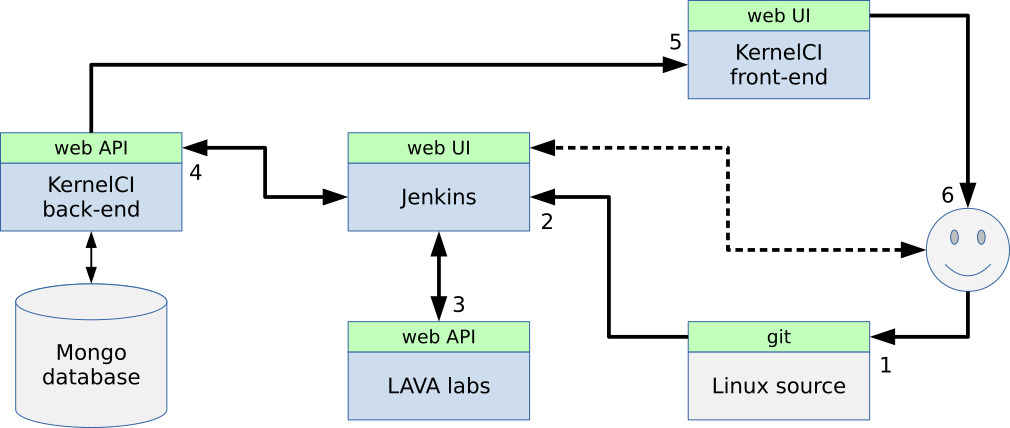
\includegraphics[width=7cm]{10_2018_Shadura1.png}
  %\caption{Блок-схема примерной системы распознавания РОГ}
  \label{Shadura1}
\end{figure}
\end{center} 

Kernel CI combines multiple components in a pipeline:
\begin{itemize}
\item New code lands in the Linux kernel Git repository
\item Jenkins triggers the build process with multiple configurations
\item After build finishes, Jenkins submits LAVA jobs
\item LAVA boots the built Linux kernels
\item Results get pushed back to Kernel CI
\end{itemize}

This process is applied to the master branch, \textbf{next} branch, stable branches and various topic branches (e.g. arm-soc, adnroid etc)

\subsection*{How to use LAVA}

There are two types of configuration files controlling LAVA: job definitions and test definitions. Job definitions tell LAVA how to get a specific series of test running on a device, i.e. what ot boot on the device, how to set up the environment and what tests to run. Test definitions define the tests themselves: what commands need to be run to get the test executed.

\subsubsection*{LAVA job definitions}

LAVA jobs are described using a YAML-based job definition\linebreak language. They define some job metadata and a series of actions. Each action tells LAVA to deploy an OS, boot it or run some tests in it. If needed, actions may repeat, so that the process consists of multiple stages.

In the simplest case, a job may look like this:

\begin{verbatim}
device_type: bcm2836-rpi-2-b
job_name: boot test
visibility: public\end{verbatim}\begin{verbatim}timeouts:
  job:
    minutes: 10\end{verbatim}\begin{verbatim}actions:
- deploy:
    to: tftp
    kernel:
      url: https://server.org/path/to/zImage
      type: zimage
    dtb:
      url: https://server.org/path/to/raspberry-pi-2b.dtb
    ramdisk:
      url: https://server.org/path/to/ramdisk-armhf.cpio.gz
      compression: gz
    os: oe\end{verbatim}\begin{verbatim}- boot:
    method: u-boot
    commands: ramdisk
    auto_login:
      login_prompt: 'root login:'
      username: root
    prompts: ['# ']\end{verbatim}This simple job just boots the kernel without running any actual tests. LAVA should already know how to boot Raspberry Pi 2 Model B given URLs to the kernel, DTB and the ramdisk. Alternatively, it can be booted from e.g. NFS filesystem.

It’s a bit more complicated when the target OS cannot be put on NFS or when you need to test the actual target images, as is the case with Apertis, a Debian derivative for automotive use. LAVA cannot boot directly into the flash or SD card image, so we need to split the boot process in two stages: the first one boots a minimal Linux system which puts the image onto a permanent storage, and then reboots into that image.

\begin{verbatim}
- boot:
    namespace: flash
    timeout:
      minutes: 10
    method: u-boot
    commands: nfs
    prompts:
    - 'root@stretch:'
    auto_login:
      login_prompt: 'stretch login:'
      username: root
      password_prompt: 'Password:'
      password: password
      
- deploy:
    namespace: system
    timeout:
      minutes: 20
    to: usb
    device: sd-card
    tool:
      prompts: ['copying time: [0-9ms\.\ ]+, copying speed 
[0-9\.]+ MiB\/sec']
    images:
      image:
        url: https://images.apertis.org/daily/18.09/
20180801.0/arm64/target/apertis_18.09-target-
arm64-uboot_20180801.0.img.gz
      bmap:
        url: https://images.apertis.org/daily/18.09/
20180801.0/arm64/target/apertis_18.09-target-arm64-
uboot_20180801.0.img.bmap
    uniquify: false
    os: ubuntu
    writer:
      tool: /usr/bin/bmaptool
      options: copy {DOWNLOAD_URL} {DEVICE}
      prompt: 'bmaptool: info'\end{verbatim}


Here, the first stage is put into a namespace called \verb@flash@, while the second one is called \verb@system@. In the first stage, LAVA deploys a minimal Debian stretch system, which contains \verb@bmaptool@, a tool which can effectively write images with big holes, which is what most OS images are. LAVA sets up a root FS to be available over NFS and boots into it, entering the next stage. In the secondary stage, \verb@deploy@ action tells LAVA to download the image and write it to the SD card using \verb@bmaptool@. Another \verb@boot@ section afterwards instructs LAVA to reboot into the newly flashed image.

\begin{verbatim}
- test:
    timeout:
      minutes: 15
    namespace: system
    name: sanity-check
    definitions:
      - repository: https://gitlab.apertis.org/
infrastructure/apertis-tests
        revision: master
        from: git
        path: common/sanity-check.yaml
        name: sanity-check-initial
      - repository: https://gitlab.apertis.org/
infrastructure/apertis-tests
        revision: master
        from: git
        path: misc/add-repo.yaml
        name: add-repo\end{verbatim}


The \verb@test@ action tells LAVA what tests to run and where to find them.

\subsubsection*{LAVA test definitions}

Test definitions specify the test metadata and tell the LAVA test runner what dependencies the test requires, what commands to run and how to parse the output.

\begin{verbatim}
metadata:
  name: check-dbus-services
  format: "Lava-Test-Shell Test Definition 1.0"
  description: "Sanity-check all installed D-Bus services"
  maintainer: "simon.mcvittie@collabora.co.uk"
  scope:
  - functional
  devices:
  - i386
  environment:
  - lava-test-shell\end{verbatim}\begin{verbatim}install:
  deps:
  - apertis-tests
  - dbus-tests\end{verbatim}\begin{verbatim}run:
  steps:
  - common/run-test-in-systemd --user=user dbus/check-
dbus-services
  - common/run-test-in-systemd dbus/check-dbus-services\end{verbatim}\begin{verbatim}parse:
  pattern: 'RESULT:(?P<result>\w+):
(?P<test_case_id>[^:]+):'
  # LAVA doesn't seem to have the concept of an expected failure,
  # so calling it skipped is the next best thing
  fixupdict:
    xfail: skip\end{verbatim}

\subsection*{Integrating LAVA}

\begin{center}
\begin{figure}[h!]
  \centering
  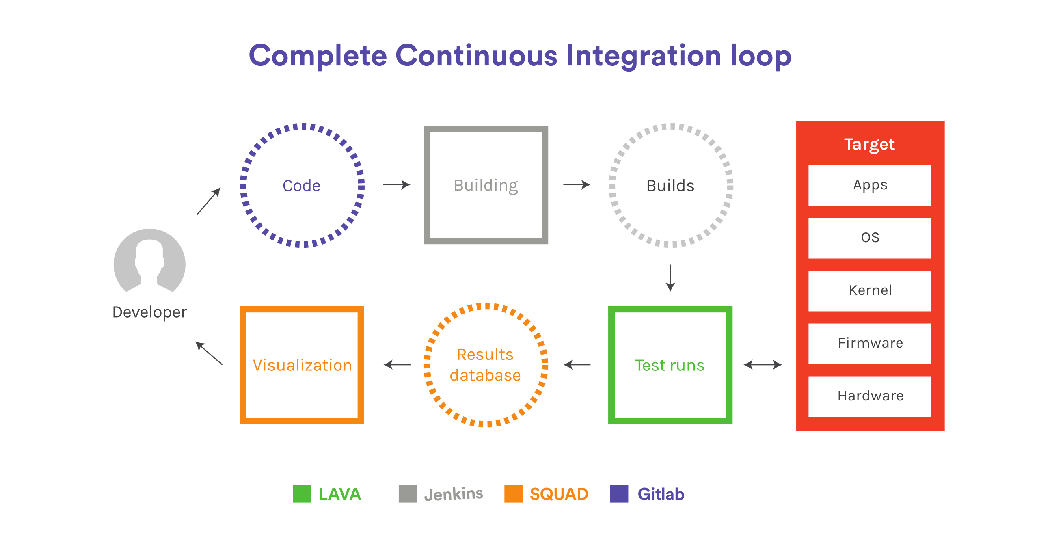
\includegraphics[width=8cm]{10_2018_Shadura2.png}
  %\caption{Блок-схема примерной системы распознавания РОГ}
  \label{Shadura2}
\end{figure}
\end{center} 

LAVA can be integrated with software such as SQUAD to store and visualise the test results. For Apertis, we have written a bridge webservice which collects results related to a series of images and posts the results to the bug tracker, and also sends email and chat notifications.

\end{document}
